\documentclass[c, aspectratio = 43]{beamer}
 \usetheme{Pittsburgh}

%%% Работа с русским языком
\usepackage{cmap}					% поиск в PDF
\usepackage{mathtext} 				% русские буквы в фомулах
\usepackage[utf8]{inputenc}			% кодировка исходного текста
\usepackage[T2A]{fontenc}			% кодировка
\usepackage[english, russian]{babel}	% локализация и переносы
%\usepackage{pscyr} % Нормальные шрифты

%%% Дополнительная работа с математикой
\usepackage{amsfonts,amssymb,amsthm,mathtools} % AMS
\usepackage{amsmath}
\usepackage{icomma} % "Умная" запятая: $0,2$ --- число, $0, 2$ --- перечисление

%% Номера формул
%\mathtoolsset{showonlyrefs=true} % Показывать номера только у тех формул, на которые есть \eqref{} в тексте.
\usepackage{gensymb}
%% Шрифты
\usepackage{euscript}	 % Шрифт Евклид
\usepackage{mathrsfs} % Красивый матшрифт

%% Свои команды
\DeclareMathOperator{\sgn}{\mathop{sgn}}

%% Перенос знаков в формулах (по Львовскому)
\newcommand*{\hm}[1]{#1\nobreak\discretionary{}
{\hbox{$\mathsurround=0pt #1$}}{}}

%%% Работа с картинками
\usepackage{graphicx}  % Для вставки рисунков
\graphicspath{{images/}{pictures/}}  % папки с картинками
\setlength\fboxsep{3pt} % Отступ рамки \fbox{} от рисунка
\setlength\fboxrule{1pt} % Толщина линий рамки \fbox{}
\usepackage{wrapfig} % Обтекание рисунков и таблиц текстом

%%% Работа с таблицами
\usepackage{array,tabularx,tabulary,booktabs} % Дополнительная работа с таблицами
\usepackage{longtable}  % Длинные таблицы
\usepackage{multirow} % Слияние строк в таблице

\beamertemplatenavigationsymbolsempty
\setbeamerfont{footline}{size=\large}
\addtobeamertemplate{navigation symbols}{}{%
	\usebeamerfont{footline}%
	\usebeamercolor[black]{footline}%
	%\hspace{1em}%
	\insertframenumber \hspace{0.5cm}
	\hyperlink{toc}{\beamerbutton{оглавление}}
}
\sloppy

\setbeamertemplate{frametitle}{\bfseries \vspace{6pt} \insertframetitle \vspace{6pt}}
  



\title{Проект по МИИАД}
\subtitle{Классификация музыкальных произведений по жанрам}
\author{Дживеликян Е.А. \\
        Латышев А.К. \\
        Сизов В.С.}
\date{4 ноября 2020 г.}
\institute[НИУ ``МФТИ'']{ Национальный исследовательский университет\\``Московский физико-технический институт''}

\begin{document}

{
	\beamertemplatenavigationsymbolsempty
	\frame[plain, noframenumbering]{\titlepage}
}
\part{Основные слайды}
\section{Датасет и инструменты}
\begin{frame}{Датасет}
    \begin{columns}
        \column{0.5\linewidth}
        \begin{itemize}
            \item 8000 треков по 30 секунд каждый, в формате .mp3
            \item 8 жанров, 1000 треков для кадого жанра
        \end{itemize}
        \column{0.5\linewidth}
        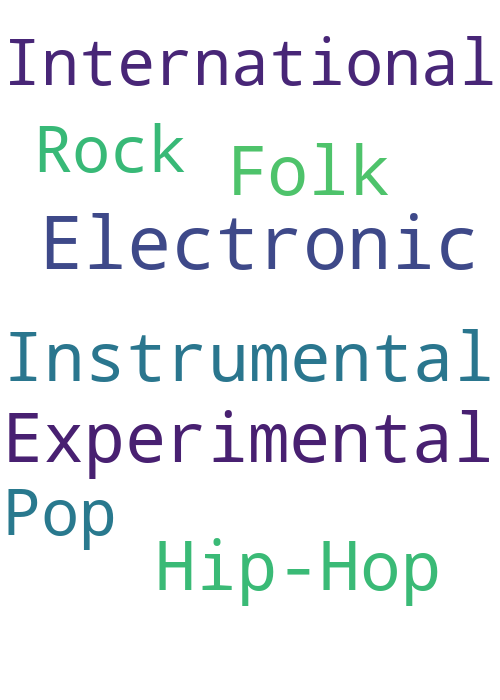
\includegraphics[width=\linewidth]{genres.png}
    \end{columns}
\end{frame}


\begin{frame}{Инструменты}
    \begin{columns}
        \column{0.5\linewidth}
        \textbf{Библиотека инструментов для обработки звука}\\
        \vspace{1cm}
        
\includegraphics[width=\linewidth]{librosa.png}
        \column{0.5\linewidth}
        \centering
        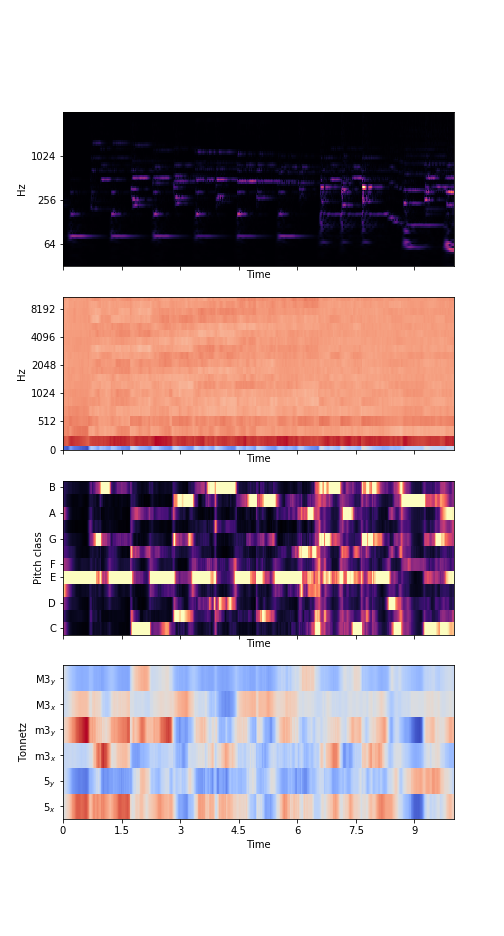
\includegraphics[height=7cm]{features.png}
    \end{columns}
\end{frame}


\section{Признаки}
\begin{frame}{Признаки}
В данной работе были использованы признаки:
\begin{itemize}
    \item MFCC(Мел-частотные кепстральные коэффициенты)
    \item Tonnetz
    \item Средний темп произведения
    \item Мощность гармонической и перкуссионной компоненты
\end{itemize}
\end{frame}

\begin{frame}{MFCC}
\centering
Спектр спектра, но по мел-шкале.\\


\begin{columns}
    \column{0.5\linewidth}
    Мел-шкала
    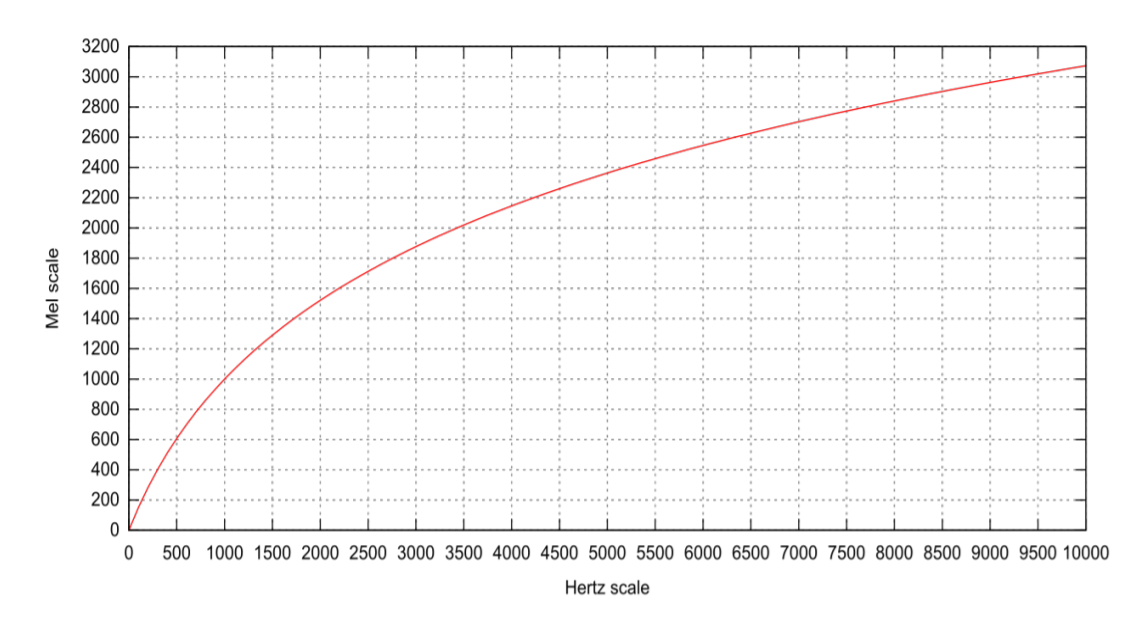
\includegraphics[width=\linewidth]{mfcc.png}
    \column{0.5\linewidth}
    Пример MFC
    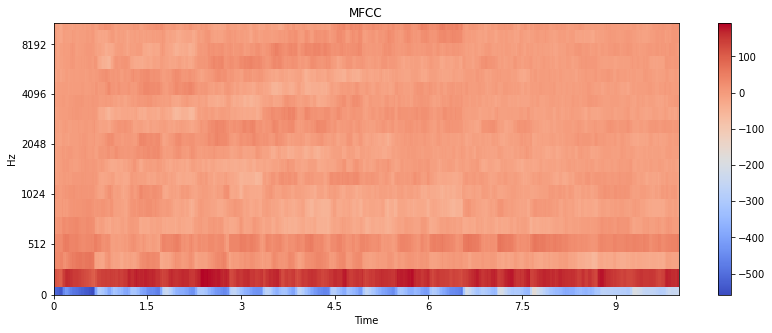
\includegraphics[width=\linewidth]{mfcc2.png}
    
\end{columns}

В датасете посчитаны 20 коэффициентов по бинам, на которые разбита песня.\\
И для каждой псоледовательности коэффициента расчитаны статистики:  mean, standard deviation, skew, kurtosis, median, minimum and maximum
\end{frame}


\begin{frame}{Tonnetz}
Данный признак позволяет оценить наличие гармонии в сигнале, выделить характерные интервалы путём преобразования пространства классов высоты звука.\\
\vspace{1cm}

\begin{columns}
    \column{0.5\linewidth}
    Пространство высот звука
    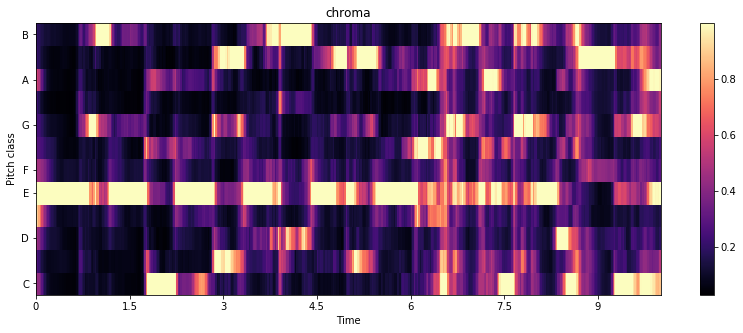
\includegraphics[width=\linewidth]{chroma.png}
    \column{0.5\linewidth}
    Пространство интервалов
    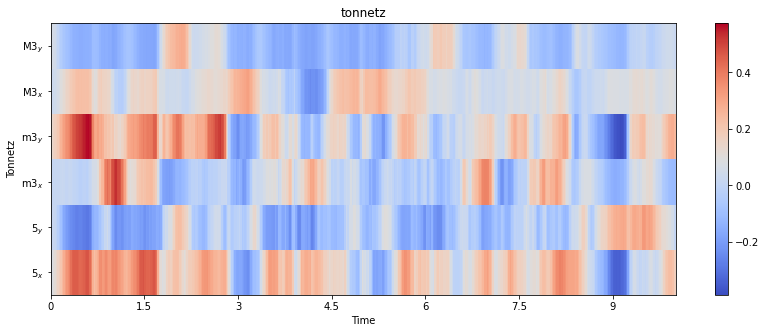
\includegraphics[width=\linewidth]{tonnetz.png}
\end{columns}
\vspace{1cm}
В данной работе используются различные статистики, вычисленные для этого признака по всем фреймам трека.
\end{frame}

\begin{frame}{Темп}
Темпоральный спектр произведения\\
\vspace{1cm}
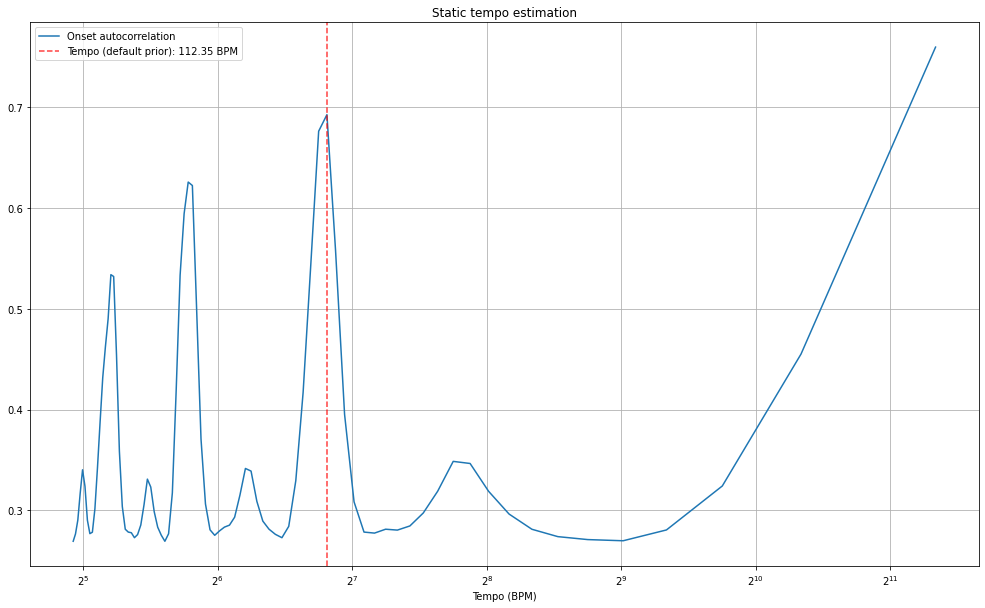
\includegraphics[width=\linewidth]{tempo.png}
\end{frame}

\begin{frame}{ГП разделение}
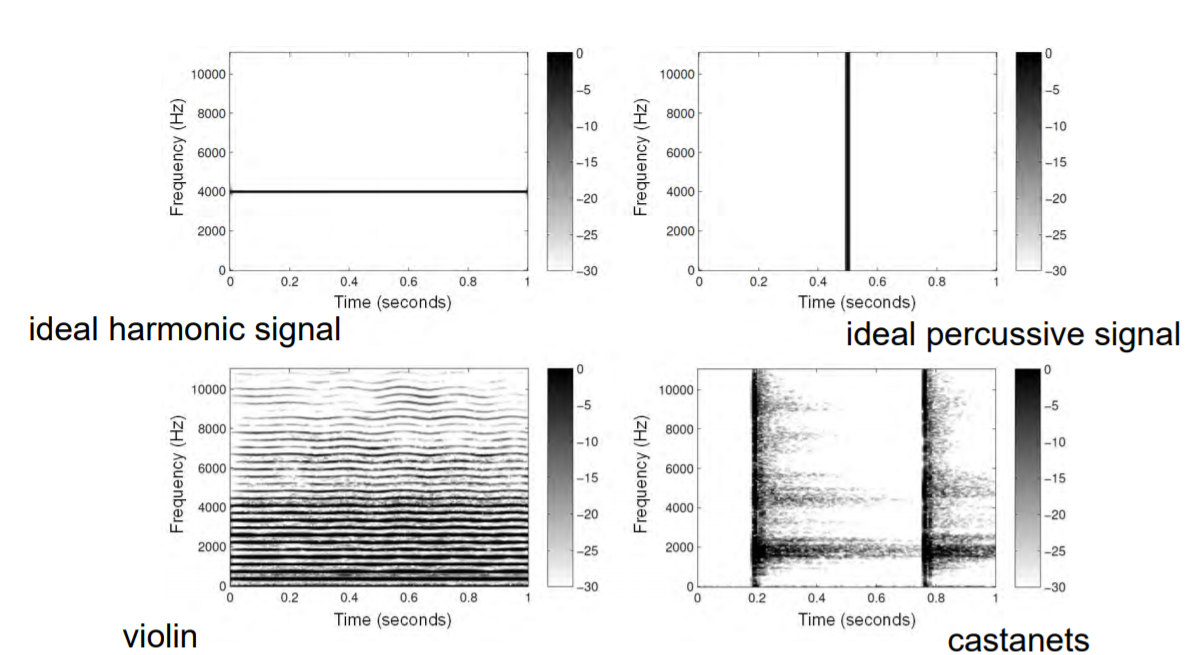
\includegraphics[width=\linewidth]{hp.png}
\vfill
Вычислены мощности гармонической и перкуссионной составляющих треков.  
\end{frame}


\section{Результаты. Часть 1}
            \begin{frame}{Результаты. Часть 1}
                      \begin{table}[]
                      \centering
\resizebox{\textwidth}{!}{
            \begin{tabular}{|c|c|c|c|c|}
            \hline
            \textbf{Модель}                                                          & \textbf{F1} & \textbf{Параметры}                                                                                             & \textbf{\begin{tabular}[c]{@{}c@{}}Время\\ обучения\end{tabular}} & \textbf{ЭВМ}                                                            \\ \hline
            SVC                                                                      & 59.92       & \begin{tabular}[c]{@{}c@{}}kernel='rbf'\\ C=3\end{tabular} & \begin{tabular}[c]{@{}c@{}}20.2 секунды\end{tabular} &  \begin{tabular}[c]{@{}c@{}}Intel(R) Xeon(R) CPU @ 2.30GHz \\ Google Colaboratory\end{tabular}                                                                      \\ \hline
            \begin{tabular}[c]{@{}c@{}}Random\\ Forest\\ Classifier\end{tabular}     & 56.23       & \begin{tabular}[c]{@{}c@{}}n\_estimators=500\\ class\_weight='balanced'\end{tabular}                           &    28 секунд &       \begin{tabular}[c]{@{}c@{}} Intel Core i9 \\ 2400 GHz  \end{tabular}     \\ \hline
            \begin{tabular}[c]{@{}c@{}}Gradient\\ Boosting\\ Classifier\end{tabular} & 57.13       & \begin{tabular}[c]{@{}c@{}}learning\_rate=0.05\\ max\_depth=5\\ n\_estimators=200\\ subsample=0.5\end{tabular} & \begin{tabular}[c]{@{}c@{}}3 минуты \\ 32 секунды\end{tabular}    & \begin{tabular}[c]{@{}c@{}}AMD Razen 5 \\ 3500U\\ 2100 MHz\end{tabular} \\ \hline
            \begin{tabular}[c]{@{}c@{}}Logistic\\ Regression \end{tabular}     &  53.22   & \begin{tabular}[c]{@{}c@{}}solver='liblinear'\\ class\_weight='balanced'\\multi\_class ='ovr'\end{tabular}                           &    46 секунд &       \begin{tabular}[c]{@{}c@{}} Intel Core i9 \\ 2400 GHz  \end{tabular}     \\ \hline
            \end{tabular}
            }
            \end{table}
\end{frame}




\section{Результаты. Часть 2}


\begin{frame}{VGG эмбеддинги}
	Для выделения признаков высокого уровня использовалась предобученная на Audioset VGG net.
	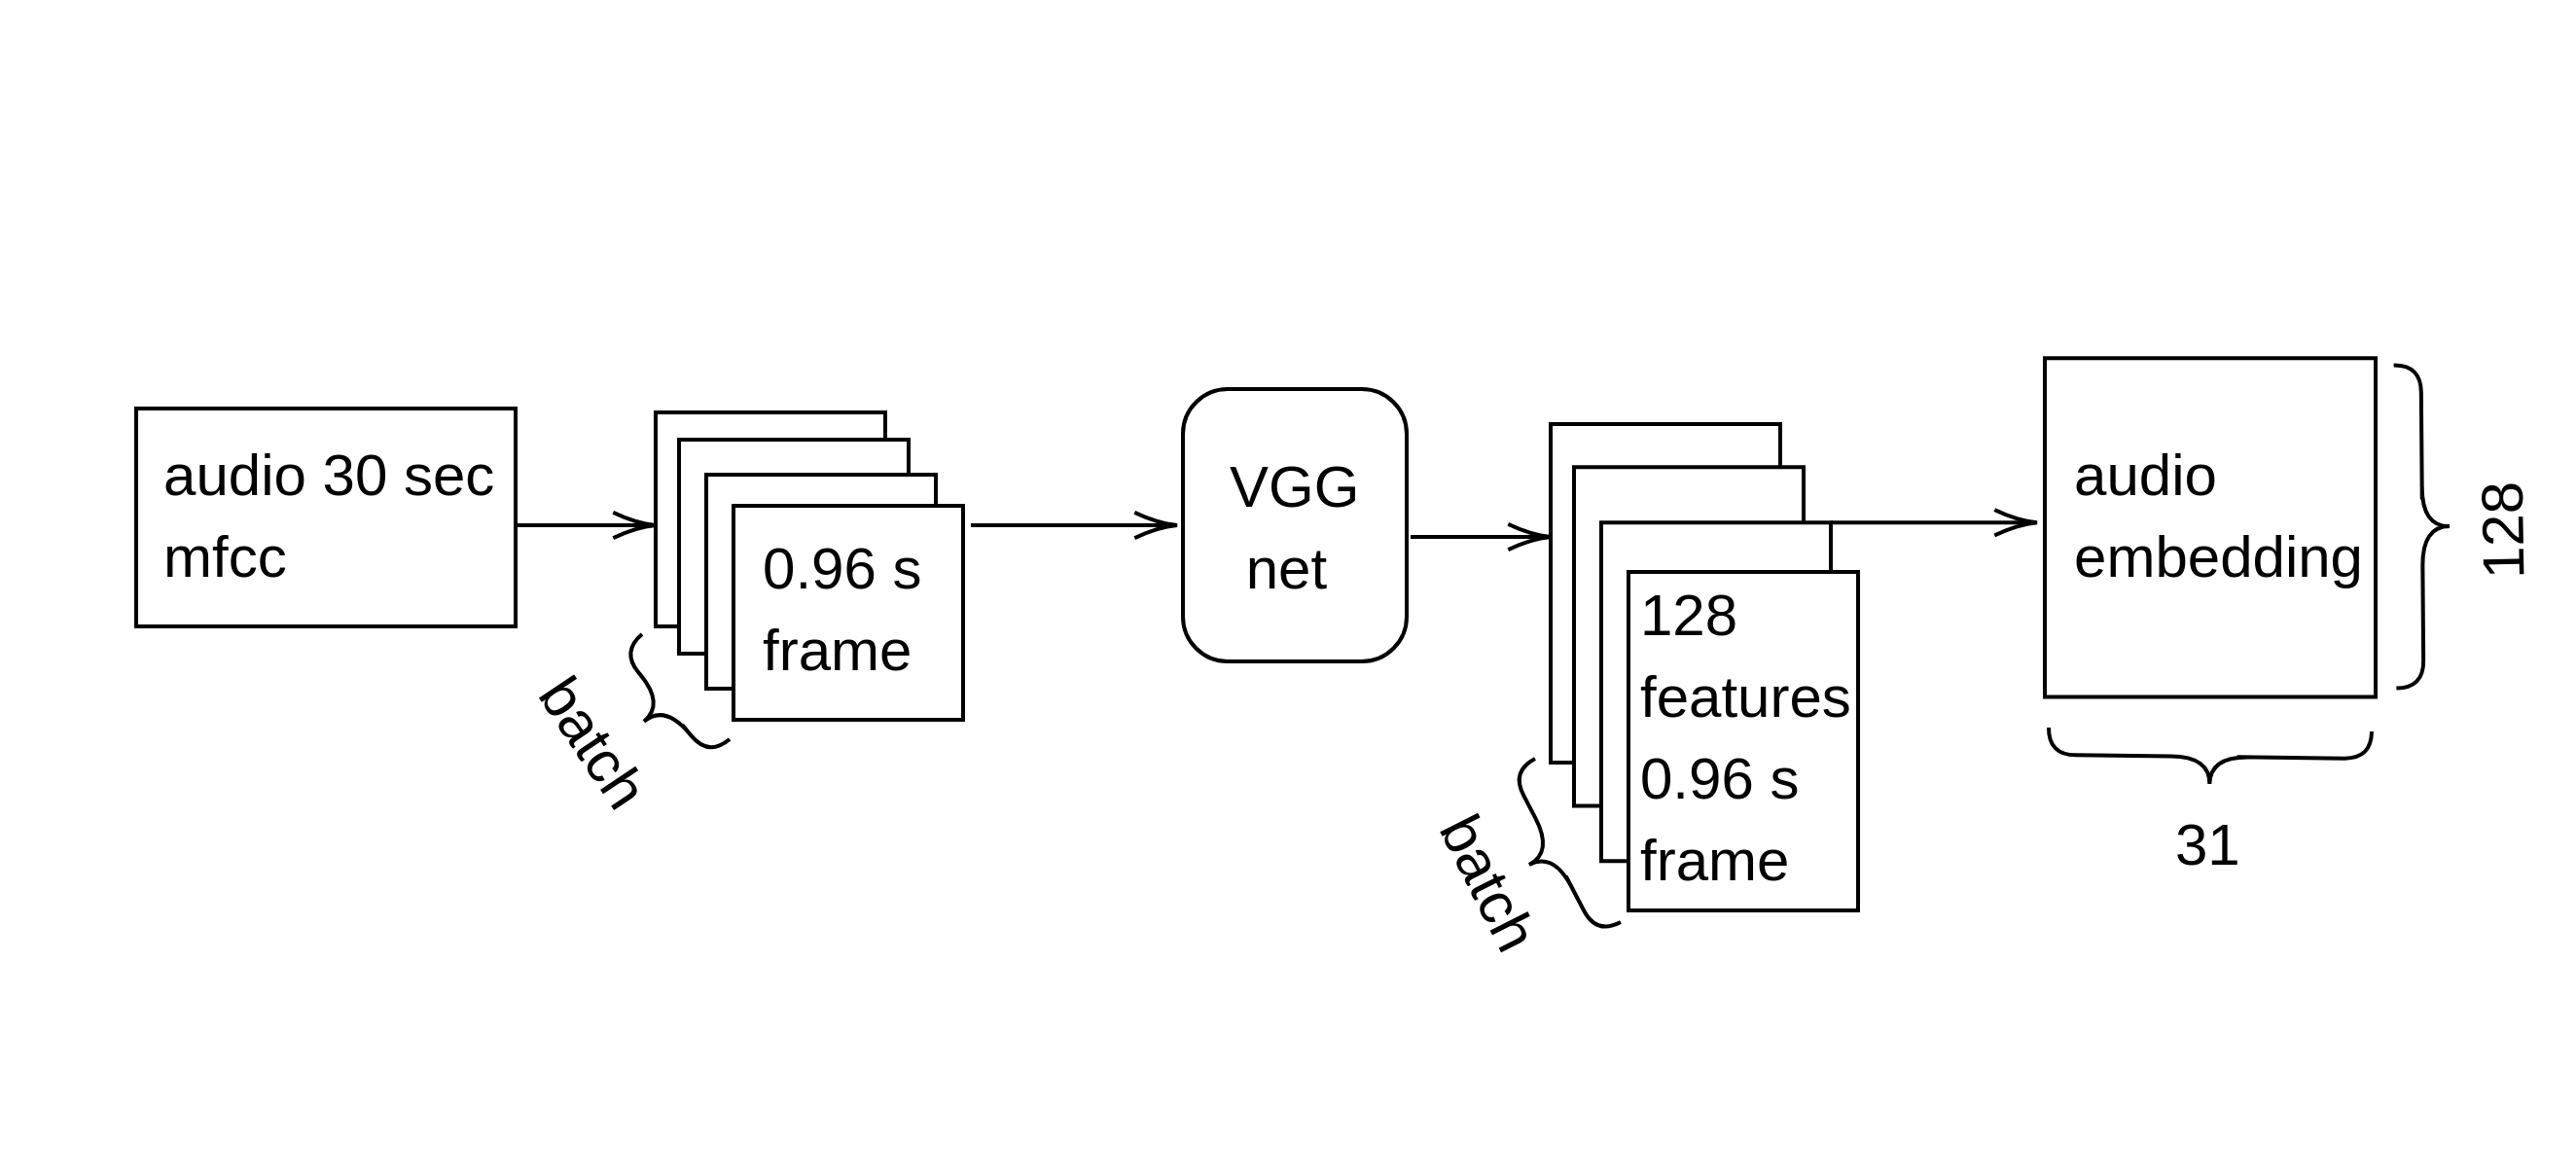
\includegraphics[width=\linewidth]{vgg_embed.png}
	VGG обучалась определять множество разных меток на 0.960 секундных отрывках на датасете Audioset, полученном из роликов youtube.
\end{frame}

 \subsection{FCNN}          
\begin{frame}{FCNN}
	
	
\end{frame}


\subsection{RNN}
            \begin{frame}{LSTM}
            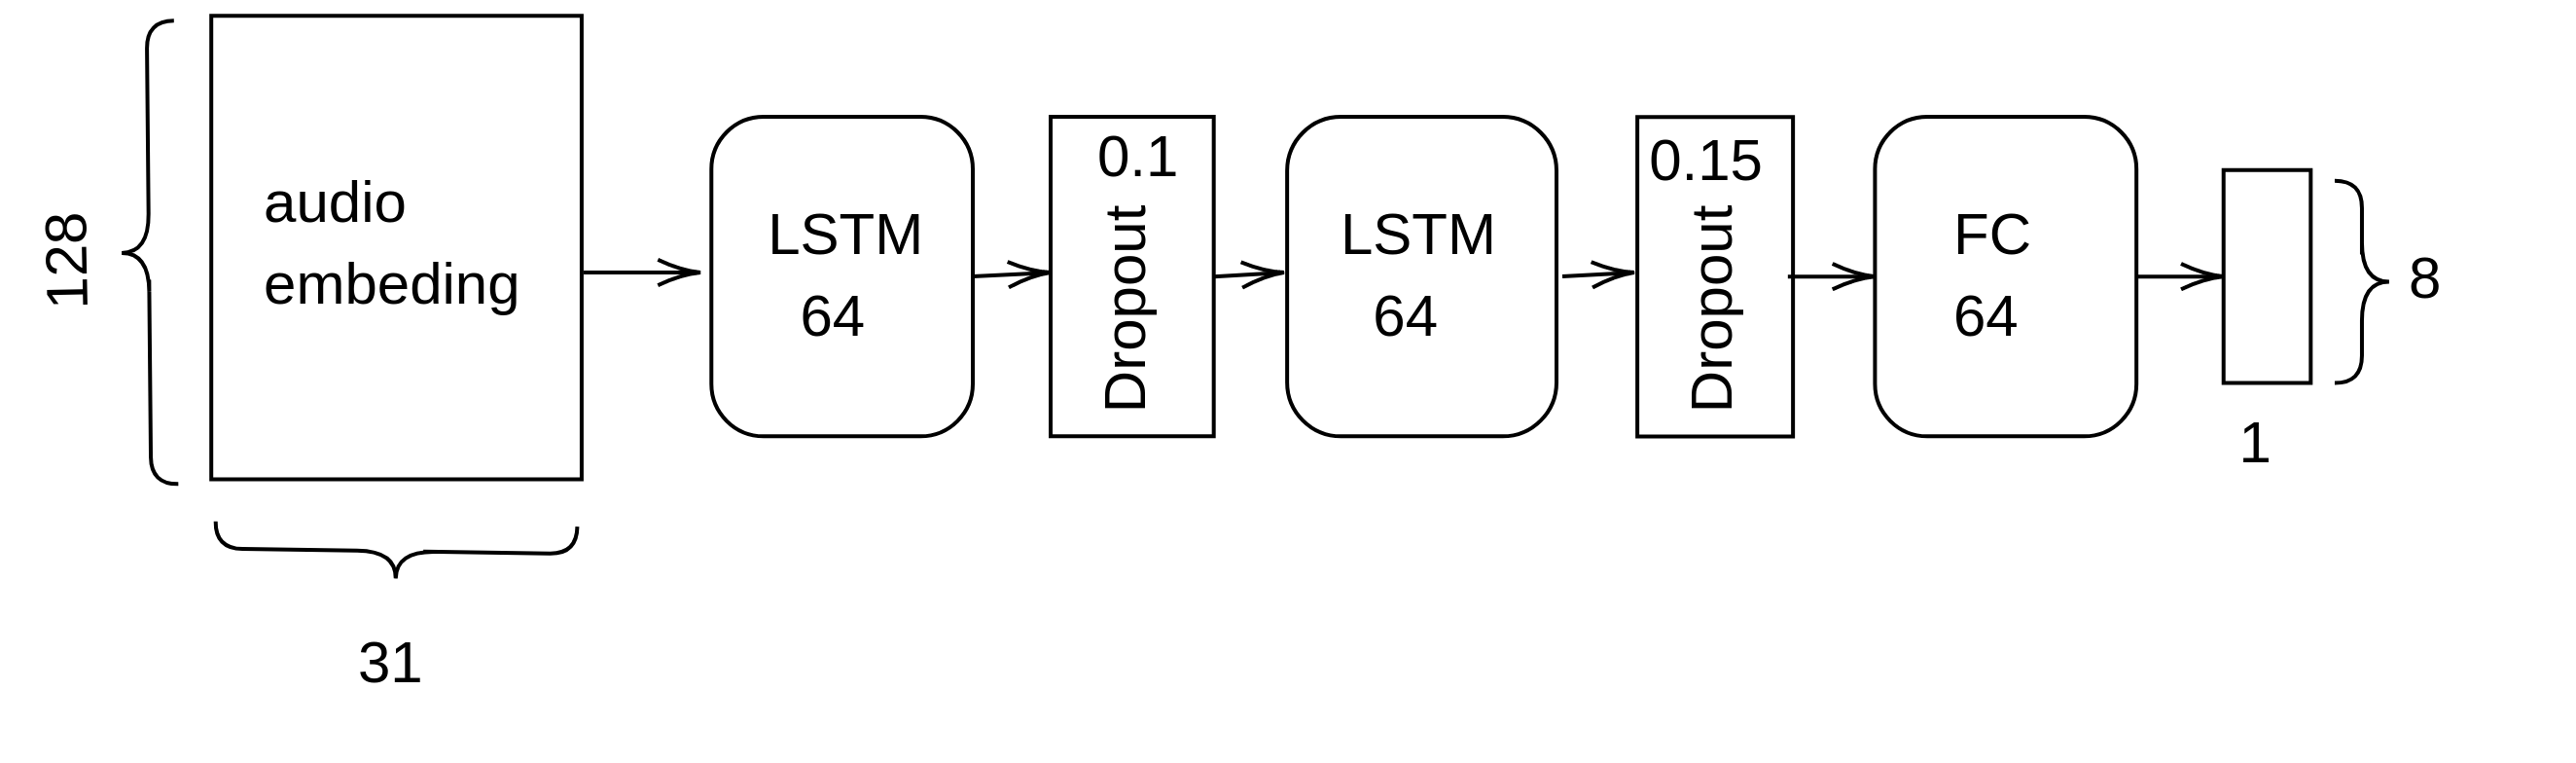
\includegraphics[width=\linewidth]{rnn_arch.png}
            \end{frame}
            \begin{frame}{Пространство поиска}
            	Сэмплировано случайным образом 200 конфигураций c помощью Ray Tune
\begin{table}[]
	\begin{tabular}{ll}
		размер скрытого слоя & \begin{tabular}[c]{@{}l@{}}от $2^3$ до $2^9$\\ с шагом степени 1\end{tabular} \\ \hline
		число слоёв          & \{1, 2, 3, 4, 5\}                                                                \\ \hline
		скорость обучения    & $(10^{-4};10^{-1})$                                                             \\ \hline
		размер батча         & \{16, 32, 64, 128, 256\}                                                         \\ \hline
		дропаут между LSTM   & $(0; 25*10^{-2})$                                                                \\ \hline
		дропаут на выходе    & $(0; 25*10^{-2})$                                                                \\
	\end{tabular}
\end{table}
Использовался ранний останов по validation accuracy и по алгоитму ASHA. 
            \end{frame}
        \begin{frame}
        	Обучение модели с лучшими параметрами
        	\begin{columns}
        	\column{0.6\linewidth}
        	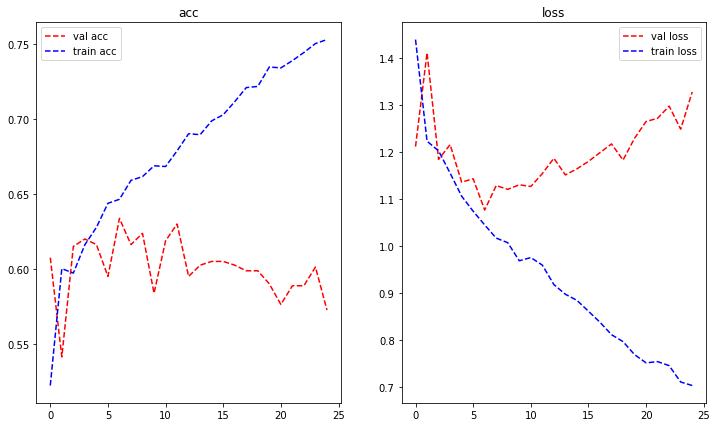
\includegraphics[width=\linewidth]{rnn_train.png}
        	\column{0.4\linewidth}
        	\begin{table}[]
        		\resizebox{\textwidth}{!}{
        		\begin{tabular}{|l|l|}
        			\hline
        			размер скрытого слоя & 64    \\ \hline
        			число слоёв          & 2     \\ \hline
        			скорость обучения    & 0.006 \\ \hline
        			размер батча         & 64    \\ \hline
        			дропаут между LSTM   & 0.1   \\ \hline
        			дропаут на выходе    & 0.15  \\ \hline
        		\end{tabular}
        	}
        	\end{table}
        \end{columns}
    Оптимизатор: Adam\\
    Функция потерь: Cross Entropy на softmax\\
    Лучший результат на тесте: 0.55 accuracy (выборка сбалансированная)
        \end{frame}
        
              \subsection{CNN}          
            \begin{frame}{CNN}
                \begin{figure}[h]
                	
\includegraphics[width=1\linewidth]{CNN.png}
                	Построенная архитектура состоит из двух сверхточных слоёв и одного линейного преобразования
                \end{figure}
            
            \begin{columns}
            
             \begin{column}{0.5\textwidth}  %%<--- here
                
                
                    \begin{center}
                     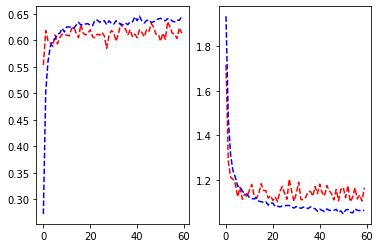
\includegraphics[width=1\textwidth]{CNN_testandval.png}
                    \tiny Слева--accuracy; справа--loss (красный--валлидация, синий--трейн)
                     \end{center}
                \end{column}
                \begin{column}{0.5\textwidth}
                   
                   
                   Количество батчей: 25\\
                   
                   
                   Результат на трейне:\\
                   Loss: 1.2092\\
                   Accuracy: 59.3333\\
                   
                   Результат на тесте:\\
                   loss: 1.299\\
                   accuracy: 0.55\\
                   
                \end{column}
               
                \end{columns}

            
            \end{frame}
% дополнительные слайды
% сделать оглавление слайдов



\beamertemplatenavigationsymbolsempty
\begin{frame}[noframenumbering]{Основные слайды}
	\hypertarget{toc}{}
	\tableofcontents[part=1]
\end{frame}

\end{document}